\documentclass[a4paper,11pt]{article}
% if you need to pass options to natbib, use, e.g.:
%     \PassOptionsToPackage{numbers, compress}{natbib}
% before loading neurips_2020

% ready for submission
%\usepackage{neurips_2020}

% to compile a preprint version, e.g., for submission to arXiv, add add the
% [preprint] option:
     \usepackage[preprint]{neurips_2020}

% to compile a camera-ready version, add the [final] option, e.g.:
%\usepackage[final]{neurips_2020}

% to avoid loading the natbib package, add option nonatbib:
%\usepackage[nonatbib]{neurips_2020}

\usepackage[utf8]{inputenc} % allow utf-8 input
\usepackage[T1]{fontenc}    % use 8-bit T1 fonts
\usepackage{hyperref}       % hyperlinks
\usepackage{url}            % simple URL typesetting
\usepackage{booktabs}       % professional-quality tables
\usepackage{amsfonts}       % blackboard math symbols
\usepackage{nicefrac}       % compact symbols for 1/2, etc.
\usepackage{microtype}      % microtypography
\usepackage{xcolor}
\usepackage{graphicx}

\title{\textcolor{red}{Generalizing from Few-Samples: COMP 691 Project Report}}

\author{%
  Nada Abdel Khalek \& Kyle Ross\\
  Department of Computer Science\\
  Concordia University\\
  Montréal, QC H3G 1M8 \\
  \texttt{\{nada.abdelkhalek, kyle.ross\}@mail.concordia.ca} \\
}
\begin{document}
\maketitle
%\begin{abstract}
%\end{abstract}
\section{Introduction}
 Deep learning has revolutionized the field of computer vision. It has notably improved the performance of image classification tasks through learning feature maps and representations, when compared to using hand-crafted features. However, the task requires an ample amount of labelled data for training networks that do not overfit. In other words, given an \textit{extremely} low amount of data, deep learning models face the inevitable problem of overfitting. In this project report, we first address the challenge of learning from a limited amount of training data with no use of external data or pre-trained models. We tackle this challenge by using a combination of classical data augmentations techniques, test-time augmentation, ensemble learning, and other regularizing methods. We also experiment with different loss functions and a recently introduced optimizer. We then address the same challenge, but without the restriction on external data and pre-trained models. We tackle this by using methods from metric based \textit{few-shot} learning tasks, and transfer learning with fine-tuning. In both challenges, we demonstrate significantly better results than the baseline and discuss other promising methods for improvement.
\section{Literature Review}
\subsection{Data Augmentation Techniques}

Data augmentation is a proven technique for increasing neural network performance, for many tasks \cite{simard1998}. Data augmentation can introduce domain priors to the training, which aid in training. For example, expert knowledge is used to define the \textit{vicinity} around each training sample, as expressed in \cite{chapelle2001}. This vicinity is used to generate new samples of the same class as the source sample. This has been applied to image classification tasks, that are renown to benefit from augmentation. Notably, when dealing with small datasets of training images, this technique is commonly used to enrich the dataset with more data. Typical augmentations for image data include horizontal reflection, rotation, and scaling, according to \cite{zhang2017mixup}, and are applied on a per dataset basis through expert knowledge. For example, the authors of AlexNet used an augmentation technique based on applying PCA to the pixel values of images, but only when training on ImageNet \cite{alexnet}. The authors of AlexNet also used \textit{random cropping}, to prevent overfitting.

In \cite{zhong2020random}, a new technique is proposed: \textit{random erasing}. This method is similar to other traditional augmentation techniques, despite being recent. It principally aims at increasing occlusion invariance in images, for training CNNs. In random erasing, a rectangular region is randomly selected from an image and replaced by random values, thereby generating various training images where the subject (or subjects) have different levels of occlusion. Random erasing is equivalent to \textit{dropout}, but for image data, as it is an extension of the \textit{cutout} technique, which is proven to also act as a regularizer \cite{cutout}. The main distinction between random erasing and cutout is that the latter only replaces square patches in an image. Moreover, the replacement colour is uniform over all pixels of the patch, instead of being noisy. This is to make the model more robust to noise, as well as occlusion.

Other recent works, such as \cite{zhang2017mixup, takahashi2018ricap}, have proposed novel data augmentation techniques to allow CNNs greater generalization capabilities. Notably, these techniques do not require additional knowledge from an expert to achieve improved performance.

In \cite{zhang2017mixup}, the authors introduce a data augmentation technique called \textit{Mixup}, in which they construct a new training example through the equivalent of alpha blending two images. This function can be expressed by the following weigthed sum: $\hat{x} = \lambda x_i + (1 - \lambda) x_j, \; \lambda \in [0,1]$, where $x_i$ and $x_j$ are samples from the training set, and $\hat{x}$ is the new image. The associated label for the new image is also given by the same function, where the inputs are ground truth one-hot encoded labels. The authors describe it formally as a random convex combination of two raw inputs, and the corresponding convex combination of the one-hot label encodings. Experiments on CIFAR-10, CIFAR-100, and ImageNet-2012 are showcased to support the claim that Mixup improves the generalization of neural networks and their robustness against adversarial examples.

In \cite{takahashi2018ricap}, the authors proposed \textit{random image cropping and patching} (RICAP) which crops four different images and patches them together to form a new training image. Using rations proportional to the area of each patch, the class labels of the four images are mixed to achieve the benefits of label smoothing. The authors evaluate the method using a WideResNet model and CIFAR-{10,100} datasets; they show consistently better results when using RICAP versus the baseline. \textcolor{red}{Maybe add some more info for RICAP here?}

In contrast to the previous approaches, A learning-based data augmentation technique called deep adversarial data augmentation (DADA) was proposed in \cite{zhang2019dada}. DADA is used to enhance the generalization ability of deep learning in extremely low data regimes. The authors formulate the problem into a class conditional supervised GAN, which does not rely on any knowledge of domain specific priors. In addition, they propose a new discriminator loss called the $2k$ loss that uses both real and augmented examples in constructing the decision boundaries. The $2k$ loss is used specifically to generate more diverse class-specific examples. Therefore, the DADA framework has $2k$ outputs unlike the vanilla GAN which has only has real/fake classes. The first $k$ outputs correspond to the probabilities of the input belonging to class $1,2,...,k$ of the real data distribution, whereas the latter $k$ outputs are probabilities for belonging to fake data. In their experiments, the authors vary the number of training images from 50 to 1000 images per class from the CIFAR-10 dataset. Moreover, they did not use any unlabelled data or any initialization from pre-training.

Similar to DADA, a learned generative model is also used in \textit{clustered optimization of latent space (COLA)} \cite{scola}. However, this model is non-adversarial and easier to train than GANs. The authors emphasize it's performance for image classification with small sample sizes, surpassing state-of-the-art methods relying on other generative models (such as GANs or VAEs) using the same datasets and no external information. COLA is first trained on the small dataset and is then used to generate new images. These new images are from classes found in the dataset and are used to create an extended training set. Half of the images in this new dataset are the original images, and the other half are synthetic. This bigger set is then used to train a classifier, such as a CNN classifier. When using only 10 samples from each class of CIFAR-10, the results show $42.86\% \pm 2.04$ testing accuracy. In comparison, the second best generative method, proposed in \cite{cfvae}, is based on a VAE and achieves $34.11\% \pm 0.67$ accuracy.

\subsection{Meta-Learning}
In the field of learning with low data regimes, the authors in \cite{olson2018modern} show that networks with as little as tens of thousands of parameters are able to generalize on small and noisy datasets. They can achieve this with minimal fine-tuning. The authors show that deep networks could be naturally interpreted as an ensemble of low-bias classifiers, whose pairwise correlations is less than one. They perform their experiments on various small datasets from the UCI repository. The median number of training examples was 601, with the smallest data set having only 10 examples. The number of features ranged from 3 to 262. Lastly, the number of classes range from 2 up to a 100. The authors compare neural networks, without dropout, to a random forest classifier.

\textit{Few-shot} learning refers to the problem of learning to generalize to previously unseen classes using \textit{few} samples during training. There are more extreme variants of few-shot learning which are \textit{one-shot} and \textit{zero-shot} learning for the cases of 1 or 0 labelled training examples per class. There are several approaches in the literature that tackle few-shot learning. The main approaches are methods based on initialization/hyper parameter tuning, metric learning, and  hallucination \cite{chen2019fewshot}. The most prominent and successful is metric learning methods \cite{ravi2016optimization}. Notable works include \textit{matching networks} \cite{vinyals2016matching}, and \textit{prototypical networks} \cite{snell2017prototypical}. 

Matching networks (MNs) are networks that tackle the one-shot learning problem by using attention as memory. Inspired by attention based memory, like in \cite{bahdanau2016neural}, MNs use a fully differentiable memory to store useful information for solving the current task. However, one difference is that memory in this architecture is non-parametric. The training procedure is based on the principle of matching the train and test conditions. By \textit{matching}, the authors aim to have the same classification performance on both seen classes, during training, and unseen classes, during testing. The goal of MNs is to learn how to \textit{learn} a classifier from a very small number of examples. Therefore, it can be thought of as a form of meta-learning. The model is trained using a support set $S$ of $k$ labelled training examples $\{x_i,y_i\}_{i=1}^k$. Given a new example $\hat{x}$ the MN calculates the probability $P(\hat{y}|\hat{x},S)$, where $P$ is the probability parameterized by the network. The estimated output label $\hat{y} = \sum_{i=1}^k a(\hat{x},x_i)y_i$ is a linear combination of all the labels in the support set $S$, where $a(.,.)$ is an attention mechanism. By using $a$, the network tries to find out how similar $x_i$ and $\hat{x}$ are. The authors define $a(.,.)$ as calculating the cosine loss between the embeddings of $g(x_i)$ and $f(\hat{x})$ and applying a softmax to normalize the distance. The embedding function $g$ is modelled as a bidirectional LSTM to encode $x_i$ by considering all elements in the support set $S$. In \cite{snell2017prototypical}, the authors interpret a MN as a weighted nearest-neighbour classifier applied within an embedding space. During training, MNs learn how to map a support set $S$ to a classification function. First a set of labels $L$ is sampled from the set of all possible labels $N$, then $L$ is used to sample a support set $S$ with a batch size of $B$. Each batch is called an \textit{episode}. The MN is trained to minimize the prediction error of the batch conditioned on the support set $S$. At test time, unlabelled examples (\textit{the query set}) are fed to the MN to make predictions. The authors perform several experiments to showcase how MNs are able to achieve state-of-the-art performance on image classification and language modelling tasks. 

\textcolor{blue}{The authors in \cite{snell2017prototypical} tackle few-shot and zero-shot learning problems by introducing prototypical networks. The proposed network learns an embedding space, in which classification can be achieved by calculating the distance between prototype representations of each class and a query point. The network learns an embedding such that points cluster around a single prototype. The prototype of a class is taken to be the mean vector of the support set in the learned embedding space. Training \textit{episodes} are a random selection of classes chosen for training, which act as the support set. The rest of the classes are kept as query points. Consequently, the classification is then performed by applying a nearest-neighbour strategy between an embedded query point and each class' prototype embedding. It has been shown that prototypical networks are equivalent to matching networks in the case of one-shot learning \cite{snell2017prototypical}. Several experiments have been showcased to prove that prototypical networks are able to achieve state-of-the-art results on CU-Birds data set. Additionally, the authors claim that prototypical networks are simpler and more efficient to implement than 2017 state-of-the-art meta-learning algorithms.}

\textcolor{blue}{Meta-learning revolves around the general idea of learning how to \texit{learn}. In meta-learning, the network tries to learn within each task, while learning about the similarities and differences between all tasks. In \cite{ravi2016optimization}, an LSTM meta-learner was used for the few-shot learning problem. The network learns a \textit{learner} through a set of datasets $\mathcal{D}$. Each dataset $\mathcal{D}_i$ has very few examples per class and is split into training $D_{train}$ and test $D_{test}$ sets. The learner tries to capture both the short term knowledge of the current task, i.e., current data set $\mathcal{D}_i$, and the long term knowledge of all the tasks in $\mathcal{D}$. Through the proposed framework the network is able to know and "task-common" initialization. The concept of the data set is equivalent to the idea of \textit{episodes} in \cite{vinyals2016matching,snell2017prototypical}. Parameter sharing is used to avoid the problem of exploding parameters. The authors make a fundamental assumption that the gradients of the learner are independent of the parameters of the meta-learner to avoid computational complexity of obtaining second derivatives. In the presented experiments, the authors used 1-shot and 5-shot classification for 5 classes, i.e., $5$-way, and they compare their results to matching networks. The results show that the proposed framework achieves much higher classification accuracy for the case of 5-shot compared with \cite{vinyals2016matching}.}

\textcolor{blue}{Similar to the idea of metric learning, in \cite{hoffer2015deep} \textit{triplet networks} were proposed. The network learns useful representations by making distance comparisons. In a triplet network, there exists three instances of the same feed-forward network. The network is fed with three samples $x,x^-$, and $x^+$, where $x$ is of the same class as $x^-$ and different from $x^+$. During training, the network attempts to fit an $L_2$ embedding using a multi-class labelled data set. However, by using such network architecture the problem essentially boils down to a  2-class classification problem, i.e., finding which of $x^- \text{or}~ x^+$ is similar to the reference $x$. The similarity is defined by the authors as sharing the label. Therefore, if $x^-$ and $x$ have the same label, the points are similar. Triplet networks learn through similarities rather than learning from labels, which could be useful in the case of hierarchical labels. The authors present several experiments on different data sets, such as CIFAR-10 and MNIST, as well as compare the performance to, their competitor at the time, Siamese networks \cite{koch2015siamese}.}

\subsection{Large Models and Transfer Learning}
In recent years, many supervised learning models have become increasingly deep and wide, thanks to mechanisms such as residual connections \cite{he2015deep}, internal memory \cite{lstm} and attention \cite{bahdanau2016neural}.

For image classification tasks, the current state-of-the-art uses such large and wide models. These are typically labelled with a \textit{-L} suffix (e.g. \textit{EfficientNet-L2}), denoting a larger variant, compared to the baseline. For example, the best performing \textit{Big Transfer} (BiT) \cite{kolesnikov2020big} and \textit{Vision Transformer} (ViT) \cite{dosovitskiy2020image} models are their largest variants.

These models require a considerable amount of labelled data. \cite{sun17} explains how the performance of CNNs is logarithmically proportional to the size of the dataset. According to experiments in \cite{dosovitskiy2020image}, the full benefits of these large networks were only observed when they use datasets such as Google's internal \textit{JFT-300M} set, which contains over 300 million images. Experiments in \cite{koch2015siamese} also support this claim. Non-flagship versions of these models also require millions of samples and train using \textit{ImageNet21k} (over 14 million images).

Fully training such models is not accessible to the average machine learning practitioner, namely due to monetary cost and time. However, as stated in \cite{kolesnikov2020big} and \cite{dosovitskiy2020image}, these networks are intended to solve new tasks using transfer learning, where the models are pre-trained and fine-tuned. 

\subsection{Vision Transformer}
The \textit{Vision Transformer} (ViT) is a recent model that attempts to bring transformers \cite{vaswani2017attention} to computer vision. Proposed in \cite{dosovitskiy2020image}, the authors implement a model that does not rely on any CNNs, which are a dominant component in most state-of-the-art vision tasks. Instead, their model is purely attention based, and therefore called a transformer. 

The ViT is not a replacement for models that use CNNs as backbones, such as ResNets \cite{he2015deep}, however. The main limitation of ViT is that the model requires a considerable amount of labeled training data. Through the authors' experiments, ViT outperforms other models when allowed a range of 14 to 300 million images. This is due to the fact that transformers lack the typical inductive biases of CNNs (namely spatial/locality bias). In other words, a transformer requires more data than a CNN, to improve generalization. 

To construct a ViT, the authors use an architecture nearly identical to original transformer introduced in \cite{vaswani2017attention}. The fundamental differences, when comparing a transformer for NLP versus vision, are found before the transformer's encoder. 

In NLP, for example, the model's input is a 1D vector of word embeddings. This vector represents a sequence of words, such as a sentence or a paragraph. The sequence is then positionally encoded, using sinusoidal function, before being fed to the transformer's encoder. The self-attention layer in the encoder allow the model to learn meaningful relationships between words, depending on their positions in sequence, thanks to the positional encoding.

When working with an image as input, a transformer's encoder still expects a sequence, where order matters. The authors of ViT propose a solution for generating a learnable sequence, based on an input image, as a key contribution. An input image is reshaped into a sequence of, smaller, square image patches, where each patch is flattened into a single channel. This is performed through a preprocessing function that maps a 2D image $\mathbf{x} \in \mathbb{R}^{H \times W \times C}$ to $\mathbf{x}_p \in \mathbb{R}^{N \times (P^2C)}$. $P^2$ is the area of the square patch, in pixels. For example, let $x \in \mathbf{R}^{32\times32\time3}$ depict a $32\times32$ image with 3 channels (RGB). Let the patch height and width be $16\times16$. 4 patches can therefore be created from $\mathbf{x}$: $N_{patches} = HW/P^2$. Each patch is flattened into a 1D vector $\in \mathbb{R}^{P^2C}$.

The Transformer's encoder expects $N+1$ inputs of fixed dimension $D$. $x_p$ is then mapped into a latent vector space of size $D$, through a linear projection $E$. The parameters of $E$ are learned. This is a distinction from the aforementioned sinusoidal approach. The added input is from a prepended \textit{[class]} token, which is learnable, as found in \cite{devlin2019bert}.

The authors name each ViT based on the breadth and depth of the model's architecture. There are 3 categories: baseline, large and huge (B, L, H). The baseline model contains the least parameters, and is tuned to support training with smaller datasets. The large variant scale up the number of parameters and layers, as it is destined to train on moderately large datasets. The huge variant is the most complex model and outperformed the other variants only when given huge datasets, such 300 million images.

Variants are also labelled with the length $P$ of the patches. Similarly to the B, L, and H labels, the patch labels is an indicator of the required resources for training. For example, the longest variant to train, which is also the best performing, is \textit{ViT-H/16}. The smaller the patch size, the more patches per images, and the more memory and compute time is necessary.

While training a ViT requires substantially less computation than training other state-of-the-art models, such as EfficientNet-L2\footnote{currently rank 1 for CIFAR-10 image classification: https://paperswithcode.com/sota/image-classification-on-cifar-10} \cite{xie2020selftraining}, training the best performing ViT remains inaccessible to most researchers. For example, training a ViT-H/14 requires 2500 TPUv3-core-days\footnote{the number of TPUv3 cores used $\times$ the training time in days.}. This is a significant improvement over the 12 300 TPUv3-core-days required to train an EfficientNet-L2, but still costly. In addition to the training time, gaining access to datasets with hundreds of millions of samples is an issue.

This training cost can be circumvented, thanks to transfer learning. The authors emphasize the relevance of using ViTs in transfer learning contexts, through experiments demonstrating how their models generally outperform others in performance versus fine-tuning cost. During this benchmark process, the authors observe a promising usage of ViTs for very low-data transfer situations, i.e, good accuracy when fine-tuning using a very small number of training samples. 

\section{Methodology}

\subsection{Challenge One}
\subsubsection{Data Preprocessing}

In the first challenge, we explore many augmentation techniques, to fight overfitting. We use traditional augmentations, as well as Mixup and RICAP. We attempted to use COLA, but there are no public implementations for this method. Despite the effort to implement the paper ourselves, we were unable to successfully do so.

We began with creating an interactive \textit{Jupyter Notebook}\footnote{https://tinyurl.com/y4nkzpx6}, using sliders, and other form elements, as an image data augmentation tool. It applies traditional augmentation techniques, powered by the \textit{imaug}\footnote{https://github.com/aleju/imgaug} library. The tool allows the user to create a subset of a large dataset, by sampling a given number of images per class. Each original sample in the subset is used to generate a given number of augmented variants. The variants are added to the subset. Each augmentation technique has a probability of being applied, when generating a new image. This allows a combination of augmentations to be applied.

We use this tool to create an augmented subset of CIFAR-10. This new set contains 100 original images from CIFAR-10, using 10 images from each of the 10 classes, along with augmented variants. We use augmentations such as horizontal flip, random erasing, slight rotations, colour temperature change, multiply, brightness, etc. Loosely inspired by daytime to nighttime image translations possible with GANs, such as \textit{Pix2Pix} \cite{isola2018imagetoimage}, we use colour temperature change, multiply, and brightness, to simulate photographs of the same subject, but taken at different times of day. We experimented with multiple ranges for the values of the augmentations, until we manually selected the combinations that yielded the best qualitative results. Figure \ref{fig:time_of_day_augmentation} depicts random examples generated using these three techniques. 

\begin{figure}[h]
    \centering
    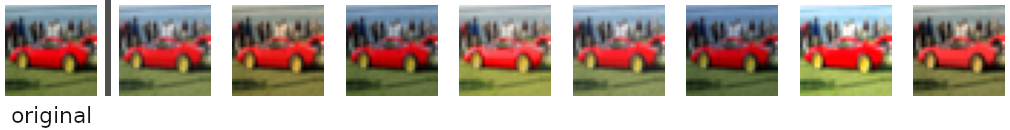
\includegraphics[width=\textwidth]{time_of_day_augment.png}
    \caption{Results of applying colour temperature change, multiply, and brightness to an original image, to simulate different times of day.}
    \label{fig:time_of_day_augmentation}
\end{figure}

This is appropriate for CIFAR-10, as most photographs within the dataset are taken outside. Images for classes such as \textit{airplane}, \textit{ship}, \textit{truck}, \textit{deer}, etc, are almost entirely taken outdoors, for example. We also use light average blurring, hoping this will help models to learn the general contour of the classes. Perceptually, blurring yields images where the shape of the subject is the most defining feature, instead of fine details. As most classes from CIFAR-10 are from very distinct categories (unlike CIFAR-100 that has many types of flowers, for example), we hypothesize that shape will be important.

To easily use this dataset with Pytorch \textit{DataLoaders}, we created our own \textit{Dataset} class \footnote{https://github.com/KyleRoss-rice/tiny-cifar10-experiments/blob/main/datasets/tinycifar10.py}. Unfortunately, we did not use this dataset, in our final version of Challenge One, as it did not work when submitting to \textit{Codalab}. 

We also created an augmentation class that helps create augmentations images on the fly. We use this class to implement Test-Time Augmentation (TTA), that is discussed furter below. \textcolor{red}{add a footnote to the class in question}

\textcolor{blue}{We use both Mixup \cite{zhang2017mixup} and RICAP \cite{takahashi2018ricap} to add more augmentations to our dataset. Mixup creates new images by using a weighted sum between two images. On the other hand, RICAP extracts four image patches and stitches them together to form a new training image. We attempt to use Mixup and RICAP as regularizers, since they will be adding supplementary noise in training training.}

\subsubsection{Architecture}
As studied in \cite{sun17}, the size of a neural network should scale up logarithmically with the number of training examples. We aim to find an architecture such that it doesn't \textit{memorize} the training data or fail to generalize, i.e. overfit to training data. Therefore, the architecture should not be too complex, i.e. have a lot of parameters. We are given only 10 samples per class, from the CIFAR-10 dataset, so the choice of the network's architecture is critical. Choosing an architecture that is too deep or wide will lead to having more parameters to learn. Hence, we adopt architectures that have 2 to 4 hidden layers or blocks. In all our proposed architectures, we chose Rectified Linear Units (ReLU) as the non-linearity, since it is the most commonly used activation in the literature, and because networks with ReLU activations are faster to train and not computationally expensive \cite{krizhevsky2012imagenet}. Furthermore, we employ batch normalization and dropout, for regularization. Dropout can also act as a proxy implementation of a ridge-type penalty, which can be used to mitigate overfitting \cite{olson2018modern}. Using dropout we will be adding a form of noise to the training, potentially making a model more robust.

In this challenge, all the models we tested are CNNs. The following is a summary of each:

\textcolor{red}{Verify that the numbers (X-Layer) reflect hidden layers, or CNN "blocks"}

\textbf{4-Layer CNN}: The first architecture we propose is a 4-layer architecture as shown in \textcolor{red}{insert figure}. We employ max pooling in the first layer to reduce computational cost, while keeping the same number of feature maps, and to make our network more translation invariant. Moreover, we use average pooling in the last layer so that the network is more stable to variability. We evaluated two variants of this architecture with and without dilated convolutions. We used dilated convolutions to increase the receptive field of our network.

\textcolor{blue}{\textbf{2-layer CNN:}
This is a shrunken version of the 4-layer CNN. We also evaluated the architecture with and without dilated convolutions.}

\textcolor{blue}{\textbf{ConvNet: We employ the CNN used in prototypical networks \cite{snell2017prototypical} and change the last layer to be a fully connected layer with 10 outputs.}}
\subsubsection{Other Techniques}
\textbf{Test-Time Augmentation (TTA)}: Augmentation is commonly used before or during training, where the original training image is transformed into several versions through rotation, flipping, blurring, etc. However, augmentation can also be used at test time. Each test image is transformed into several versions and fed to the model. The model outputs the softmax prediction for each. Then, the predictions of the transformed images are averaged. This technique is called Test-Time Augmentation (TTA). We employed TTA to get "smoothed" predictions for each test image and its corresponding augmentations. It has been shown that TTA leads to greater robustness, and improved accuracy \cite{shanmugam2020and}. TTA is an appealing approach since its implementation does not require additional data and requires no change to the current model.

\textcolor{blue}{\textbf{Ensemble Deep Learning}: To have greater capacity, and to make predictions more accurate, we decided to combine the proposed architectures into an ensemble. The architecture was trained separately on the same data then at test time, we feed each model the same test data and average their softmax predictions before making a decision.}

\textcolor{blue}{\textbf{SAM}: Sharpness-Aware Minimization (SAM) is a new optimization technique, introduced in \cite{foret2020sharpnessaware}. Instead of optimizing only the training loss, it optimizes loss value and loss \textit{sharpness}, by formulating optimization as a minimax problem. Gradient descent is performed on this new formulation, using an optimizer such as SGD or Adam. For the models we were able to implement it with, we obtain better results using SAM+Adam, than using SAM+SGD, or any other optimizer without SAM. The authors claim it improves generalization across image classification tasks (namely CIFAR-10), which motivated our usage of it. The current top ranking classifier\footnote{https://paperswithcode.com/sota/image-classification-on-cifar-10} for CIFAR-10 uses SAM, for example.}

\subsection{Challenge Two}
\textcolor{red}{Talk about the learn2learn library and code used in prototypical networks from \cite{Arnold2020-ss} }
\subsubsection{Transfer Learning}
\subsubsection{Few-Shot Learning}
\clearpage
\section{Results}
\textcolor{blue}{Throughout all of our experiments for challenges 1 and 2, we use two testing sets: Test set I and Test set II. Test set I is comprised of 2000 samples taken from the CIFAR-10 train data. On the other hand, test set II contains 2000 samples from CIFAR-10 test data. For the final evaluation of our top two approaches, we sample three different instances of 2000 samples for each test set.}
\subsection{Challenge One}
\textcolor{blue}{In this section, we conduct several experiments and show case our extensive analysis and results. Our first set of experiments are tailored towards obtaining appropriate hyperparameters for \textit{ConvNet}. Our second set of experiments is targeted towards comparing the classification performance of \textit{ConvNet} to an ensemble of models.}

\textcolor{blue}{Unless otherwise specified, we use a SAM optimizer with an Adam base (SAM+Adam) at a learning rate of 1e-3 for 100 epochs. Our loss function is chosen to be the cross entropy loss. For evaluation, we chose to run over 1 instance of both test set I and II to avoid longer run times. We believe that the results will give a rough indicator to decide on the values of our hyperparameters. }\textcolor{red}{discuss batch size}

\textcolor{blue}{The augmentation technique and optimizer were varied to find their effect on the classification performance of \textit{ConvNet}. Table.~\ref{Table:convnet_optimizer_aug} summarizes our experimental results. The obtained results shows that the top optimizers were Adam and SAM+Adam. However, when it came to the augmentation technique our results weren't strongly conclusive. Although, we found that heavy classical augmentations did more harm than good, a moderate amount of classical augmentations gave the right amount of noise to the training and helped regularize the model.}

\begin{table}[h!]

\begin{center}
\caption{The effect of changing the augmentation technique and optimizer on the testing accuracy of ConvNet while keeping the lr=1e-3 for 100 epochs (over 1 instance).}
\begin{tabular}{|c|l|l|l|l|l|l|}
\hline
                          & \multicolumn{3}{c|}{Test set I}      & \multicolumn{3}{c|}{Test set II}     \\ \hline
\multicolumn{1}{|l|}{Augmentation} & RICAP   & Mixup   & Classical        & RICAP   & Mixup   & Classical        \\ \hline
Adam                               & 32.30\% & 34.00\% & 33.90\%          & 31.00\% & 31.40\% & 33.15\%          \\
SGD                                & 29.40\% & 30.15\% & 29.20\%          & 29.20\% & 28.50\% & 29.30\%          \\
SAM+Adam                           & 33.05\% & 33.60\% & \textbf{35.20\%} & 31.40\% & 32.50\% & \textbf{34.20\%} \\
SAM+SGD                            & 28.75\% & 28.20\% & 29.55\%          & 28.35\% & 27.40\% & 28.65\%          \\ \hline
\end{tabular}
\end{center}
\label{Table:convnet_optimizer_aug}
\end{table}
\textcolor{blue}{To study the effect of changing $\beta$ (used to do RICAP augmentations) on the performance of \textit{ConvNet}, $\beta$ was varied and the classification performance was measured on test set I and II. In Table.~\ref{table:convnet_beta}, our results show that using a $\beta=$ 1e-2 yielded the best performance. \textcolor{red}{In appendix A}, we have complementary experiments that show the effect of $\beta$ on the convergence of SAM+Adam. Our results suggest that $\beta=$1e-2 encourages the optimization algorithm to converge faster.}\textcolor{red}{Include discussion from the paper on how the choice of $\beta$ is important.}
\begin{table}[h!]
\caption{The effect of different $\beta$ on the test performance of ConvNet when using RICAP augmentation using SAM+Adam optimizer with a lr=1e-3 for 100 epochs (using 1 instance).}
\begin{center}
\begin{tabular}{|l|l|l|}
\hline
$\beta$ & Test set I & Test set II \\ \hline
1e-2    & \textbf{32.55\%}    & \textbf{32.80\%}     \\
1e-1    & 32.75\%    & 31.95\%     \\
1       & 31.70\%    & 29.65\%     \\
1e1     & 29.15\%    & 27.50\%     \\ \hline
\end{tabular}
\end{center}
\label{table:convnet_beta}
\end{table}


\textcolor{blue}{Finally, we examine the effect of different learning rates on the SAM+Adam optimizer, while using only Mixup augmentations. From Table.~\ref{Table:learning_rates_convnet} we conclude that lr=1e-3 and lr=1e-4 are good candidates for running our final experiments.}

\begin{table}[h!]
\caption{The effect of changing the learning rate with different optimizers while using mixup as an augmentation technique on the test accuracy of ConvNet for 100 epochs (using 1 instance).}
\begin{center}
\begin{tabular}{|c|l|l|l|l|l|l|}
\hline
                                    & \multicolumn{3}{c|}{Test set I}      & \multicolumn{3}{c|}{Test set II}     \\ \hline
\multicolumn{1}{|l|}{Learning Rate} & 1e-3    & 1e-4             & 1e-5    & 1e-3    & 1e-4             & 1e-5    \\ \hline
Adam                                & 29.10\% & \textbf{32.80\%} & 26.90\% & 29.15\% & 31.85\%          & 25.00\% \\
SGD                                 & 29.65\% & 18.75\%          & 7.35\%  & 28.95\% & 17.00\%          & 7.85\%  \\
SAM+Adam                            & 32.30\% & 32.45\%          & 25.15\% & 31.50\% & \textbf{32.75\%} & 23.90\% \\
SAM+SGD                             & 28.60\% & 17.85\%          & 7.55\%  & 27.40\% & 16.60\%          & 8.40\%  \\ \hline
\end{tabular}
\end{center}
\label{Table:learning_rates_convnet}
\end{table}
\newpage

\textcolor{blue}{For the rest of this subsection, we focus on two main approaches to challenge one, the first being training of an ensemble of models and the second being training of an individual model namely \textit{ConvNet}. Keeping in mind all conclusions from the previous experiments, we use SAM+Adam optimizer at a learning rate of 1e-3. We train for 200 epochs using classical augmentations and RICAP with a $\beta$= 5e-2, then continue the training for 100 more epochs using classical augmentations and Mixup. Similar to the previous experiments, we chose our loss function to be the cross entropy loss. We decided to train with all three augmentation techniques, because we believe that by doing so the models will have enough noisy training data and thus decreasing our chances of over-fitting. We train the four proposed architectures \textit{4-layer CNN}, \textit{4-layer Dilated CNN}, \textit{2-layer Dilated CNN}, and \textit{ConvNet} individually. We were interested in comparing the test performance of an ensemble of models to that of an individual model. We use all of the four architectures to construct our ensemble. During test time, the predictions of the trained models are averaged and the predicted label is decided based on those averaged predictions. The training loss, training accuracy, training run time, and testing run time were measured for both proposed approaches. A curve smoothing function, that implements a convolution window to do the smoothing, was used to make the training curves neater for analysis.} \textcolor{red}{discuss batch size}

\textcolor{blue}{In Fig.~\ref{fig:training_runtime_ch1}, we show the training loss and training accuracy over epochs along with the train and test run times. Examining the training loss curves, there is a general decreasing trend in the loss, however, at about epoch 200 the loss starts to increase again and this is because the augmentation technique has been changed from RICAP to Mixup. Through inspecting the bar graph on the right of Fig.\ref{fig:training_runtime_ch1}, it is clear that using an ensemble of models heavily increases the train run time, making our ensemble about 7.9x slower than the testbed benchmark. However, by using only \textit{ConvNet} the train run time is only 3.26x slower than the testbed benchmark. Table.~\ref{Table:best_models_challenge1} summarizes the test results using both approaches. Therefore, we conclude that by using \texit{ConvNet} the train run time is $\sim$ 2.43x faster than using an ensemble and increases the testing performance by $\sim$ 2\% on average on both test set I and II.}

\begin{figure*}[h!]
    \centering
    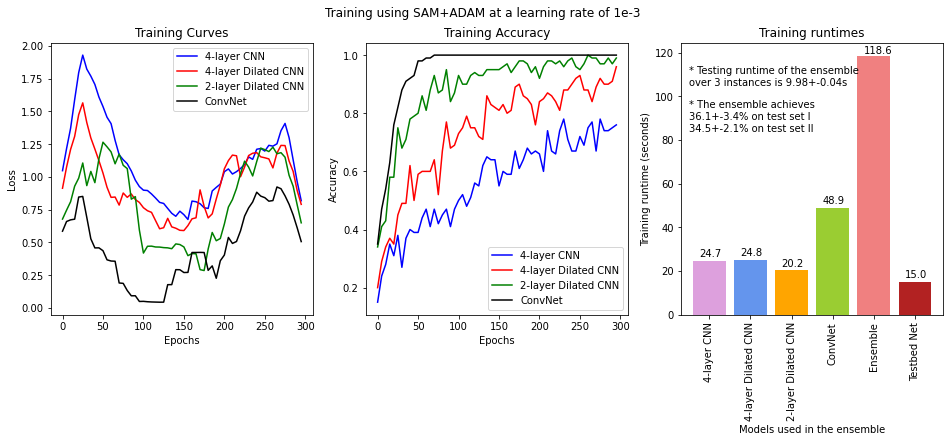
\includegraphics[width=1\linewidth]{best_performing_model_training_test_curves.png}
    \caption{The training loss curves, training accuracy curves, and training run times for models used in the ensemble in challenge one.}
    \label{fig:training_runtime_ch1}
\end{figure*}
\begin{table}[t!]
\caption{Our top two performing approaches for challenge one.}
\begin{center}
\begin{tabular}{|l|l|l|}
\hline
         & Test set I             & Test set II            \\ \hline
Ensemble & 36.1+-3.45\%           & 34.5+-2.14\%           \\
ConvNet  & \textbf{38.25+-3.08\%} & \textbf{36.25+-3.08\%} \\ \hline
\end{tabular}
\end{center}
\label{Table:best_models_challenge1}
\end{table}
\subsection{Challenge Two}
For challenge two we focus on two upper level ideas: Transfer learning, and Few-shot learning. 
\subsubsection{Transfer Learning}
\textcolor{blue}{
In this subsection we explore transfer learning in depth. Five candidate models, pretrained on ImageNet, were chosen for our experiments. We aim to explore the effect of the choice of optimizer, learning rate, and data augmentations on the effectiveness of transfer learning. Models such as \textit{VGG16}, \textit{GoogleNet}, and \textit{ResNext50} were loaded from Pytorch hub. However, the pretrained ViT model was loaded using Luke Melas-Kyriazi's GitHub repository \cite{vit_github}. Similarly, the pretrained \textit{SE-ResNet50} model was loaded from Ryuichiro Hataya's GitHub repository \cite{se_resnet_github}. The final layer of all models was changed to fit our classification problem of 10 classes. All of the parameters except the last layer were set to not requiring gradients to avoid having memory issues. To conduct controlled experiments, the number of training epochs was set to 10.  Only the parameters of the last layer passed to the optimizer to be trained using the 100 training data sample only. The loss function was chosen to be the cross entropy loss.}

\textcolor{blue}{Studying the effect of the learning rate on the classification performance of the models, an SAM+Adam optimizer is used and the learning rate was varied. The classification accuracy is assessed using test set I. Our results in Table.~\ref{Table:challenge2_optimizer_rate} show that the best classification performance is attained by training the ViT model using SAM+Adam at a learning rate of 1e-2. Decreasing the learning rate led to performance degradation for the same number of training epochs. Furthermore, we explore the effect of the type of optimizer on the classification performance. The type of optimizer was varied and the classification performance was measured using test set I. Table.~\ref{Table:challenge_2_optimizer} summarizes the obtained results. We deduce that training the last layer of the ViT model at a learning rate of 1e-3 using SAM+RMSprop achieved the best classification performance of 89.1+-1.1\% in the 10 epochs of training. Almost the same classification is achieved by using SAM+Adam optimizer at a learning rate of 1e-2 for the same number of training epochs. }
\begin{table}[h!]
\centering
\caption{Classification performance of the candidate models on test set I.}
\label{Table:challenge2_optimizer_rate}
\begin{tabular}{|c|l|l|l|} 
\hline
                                                         & \multicolumn{3}{c|}{SAM+Adam}                                                      \\ 
\hline
\begin{tabular}[c]{@{}c@{}}Learning \\ rate\end{tabular} & \multicolumn{1}{c|}{1e-2} & \multicolumn{1}{c|}{1e-3} & \multicolumn{1}{c|}{1e-4}  \\ 
\hline
VGG16                                                    & 46.1+-12.2\%              & 54.8+-5.8\%               & \textbf{68.8+-3.1\%}       \\
GoogleNet                                                & 50.5+-9.9\%               & 60.7+-6.3\%               & 20.3+-6.7\%                \\
ViT                                                      & \textbf{89.0+-0.8\%}      & \textbf{83.5+-5.1\%}      & 28.4+-10.7\%               \\
ResNext50                                                & 35.1+-3.8\%               & 61.1+-6.5\%               & 34.7+-9.2\%                \\
SE-ResNet50                                              & 44.0+-6.9\%               & 63.1+-4.4\%               & 31.9+-10.4\%               \\
\hline
\end{tabular}
\end{table}

\begin{table}[h!]
\caption{The effect of changing the optimizer with a lr=1e-3 on the classification performance of the candidate models measured on test set I.}
\begin{tabular}{|c|l|l|l|l|l|l|}
\hline
            & \multicolumn{1}{c|}{\begin{tabular}[c]{@{}c@{}}SAM\\ +Adam\end{tabular}} & \multicolumn{1}{c|}{\begin{tabular}[c]{@{}c@{}}SAM\\ +SGD\end{tabular}} & \multicolumn{1}{c|}{\begin{tabular}[c]{@{}c@{}}SAM\\ +RMSprop\end{tabular}} & \multicolumn{1}{c|}{\begin{tabular}[c]{@{}c@{}}SAM\\ +Adadelta\end{tabular}} & \multicolumn{1}{c|}{Adam} & \multicolumn{1}{c|}{SGD} \\ \hline
VGG16       & 54.8+-5.8\%                                                              & \textbf{27.8+-8.3\%}                                  & 48.4+-17\%                                                                  & 11.3+-1.1\%                                                                  & 49.4+-5.3\%               & \textbf{48.4+-7.9\%}     \\
GoogleNet   & 60.7+-6.3\%                                                              & 8.0+-0.9\%                                                              & 64.6+-2.0\%                                                                 & 9.1+-0.36\%                                                                  & 60.3+-7.6\%               & 13.9+-2.6\%              \\
ViT         & \textbf{83.5+-5.1\%}                                    & 13.4+-0.5\%                                                             & \textbf{89.1+-1.1\%}                                       & 8.4+-0.2\%                                                                   & \textbf{84.1+-5.7\%}      & 18.1+-1.2\%              \\
ResNext50   & 61.1+-6.5\%                                                              & 10.8+-1.6\%                                                             & 56.7+-6.4\%                                                                 & 8.6+-0.56\%                                                                  & 67.0+-4.6\%               & 16.8+-3.4\%              \\
SE-ResNet50 & 63.1+-4.4\%                                                              & 13.2+-0.9\%                                                             & 60.6+-3.4\%                                                                 & \textbf{14.1+-0.70\%}                                       & 63.3+-4.1\%               & 19.7+-3.2\%              \\ \hline
\end{tabular}
\label{Table:challenge_2_optimizer}
\end{table}

\textcolor{blue}{In Fig.~\ref{fig:Training_curves_ch2best}-\ref{fig:Training_curves_ch2_e-4} we study the optimization convergence under different learning rates while using a SAM+Adam optimizer. By examining the loss curves in Fig.\ref{fig:Training_curves_ch2best}, it can be noticed that a learning rate of 1e-2 is quite high causing the training to be unstable (not converging). However, the loss curves of the other models enjoy a more stable general decreasing trend. It is quite apparent that the ViT model surpasses all other models, as it converges faster to a lower loss and has a higher training accuracy than any other model. We can see from the bar chart on the right of Fig.~\ref{fig:Training_curves_ch2best} that the ViT model achieves the highest testing accuracy on test set I, almost double the accuracy of any other model. Comparing Fig.~\ref{fig:Training_curves_ch2_e-3} and Fig.~\ref{fig:Training_curves_ch2best}, we can notice that the training is stable for all models, however the VGG16 model over-fits quite fast compared to the other models. Again, we notice that the ViT model's classification performance surpasses all other models. Finally, in Fig.~\ref{fig:Training_curves_ch2_e-4} the learning rate is quite slow for all other models except VGG16. In fact, at this learning rate, VGG16 outperforms all other models with almost double the accuracy percentage. }

\begin{figure}[h!]
    \centering
    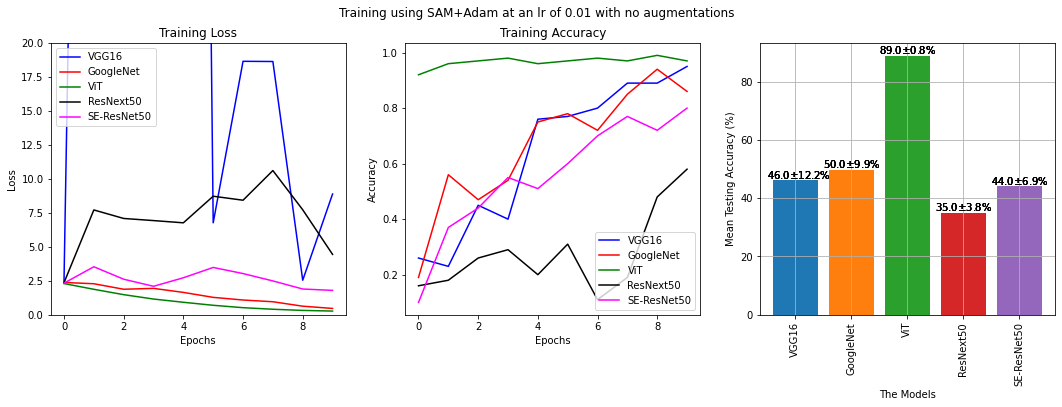
\includegraphics[width=0.8\textwidth]{Best_soln_for_challenge2.png}
    \caption{Training loss, training accuracy, and testing accuracy on test set I using SAM+Adam optimizer at a lr=1e-2 for 10 epochs.}
    \label{fig:Training_curves_ch2best}
\end{figure}
\begin{figure}[h!]
    \centering
    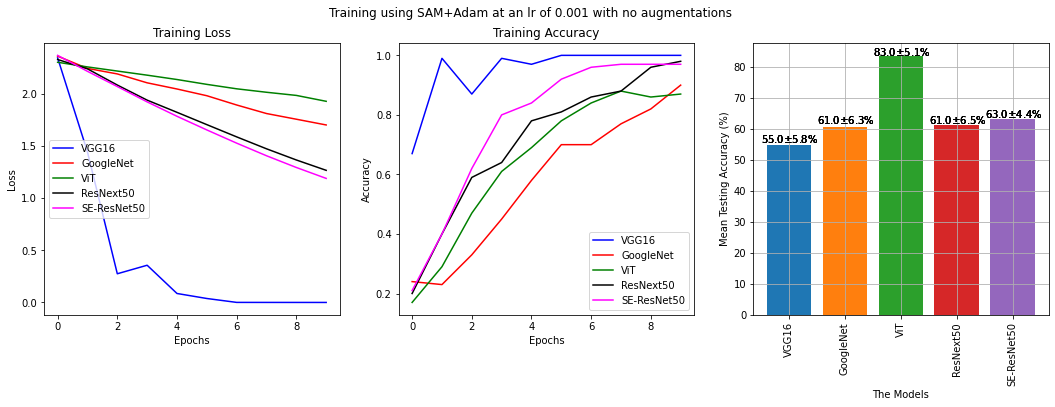
\includegraphics[width=0.8\textwidth]{SAM+Adam_lr0.001.png}
    \caption{Training loss, training accuracy, and testing accuracy on test set I using SAM+Adam optimizer at a lr=1e-3 for 10 epochs.}
    \label{fig:Training_curves_ch2_e-3}
\end{figure}
\begin{figure}[h!]
    \centering
    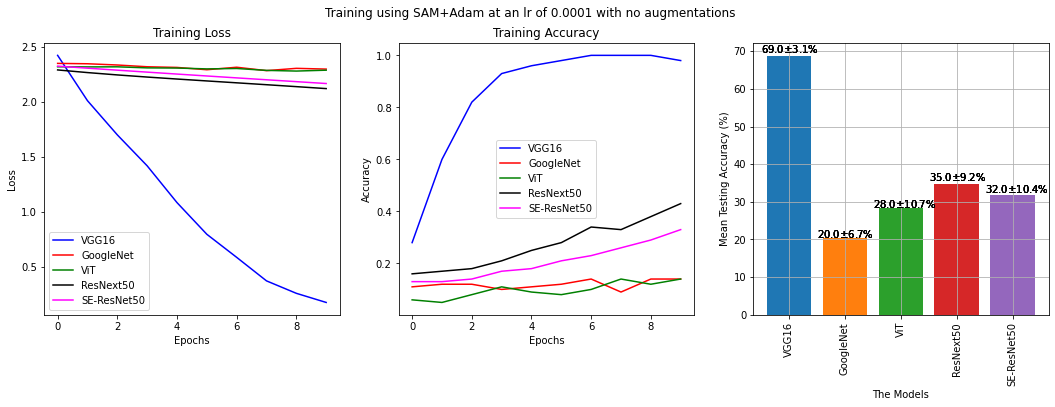
\includegraphics[width=0.8\textwidth]{SAM+Adam_lr0.0001.png}
    \caption{Training loss, training accuracy, and testing accuracy on test set I using SAM+Adam optimizer at a lr=1e-4 for 10 epochs.}
    \label{fig:Training_curves_ch2_e-4}
\end{figure}
\clearpage
\begin{figure}[t!]
    \centering
    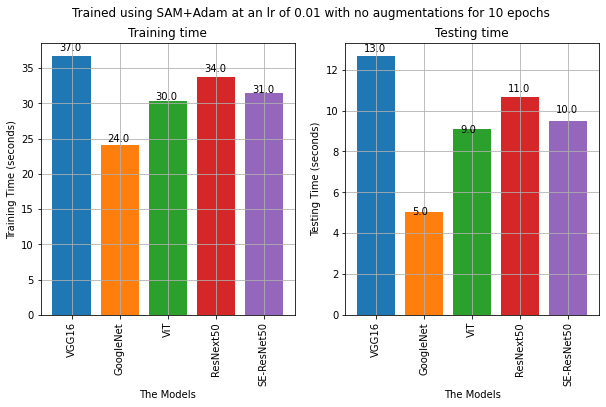
\includegraphics[width=0.5\textwidth]{best_soln_time.png}
    \caption{Train and test run times using a SAM+Adam optimizer at a lr=1e-2 for 10 epochs.}
    \label{fig:Training_curves_ch2_best_time}
\end{figure}

\textcolor{blue}{To measure the train and test run times, we trained the last layer of each model using SAM+Adam at a learning rate of 1e-2. It can be noticed in Fig.~\ref{fig:Training_curves_ch2_best_time} that VGG16 takes the most time to train, while GoogleNet takes the least amount of training time. \textcolor{red}{insight on why this happens?}}

\textcolor{blue}{Finally, in Table.~\ref{Table:Best_challenge2} we compare the classification performance of our best model namely the ViT model against the other models. Our results show that the ViT model trained with SAM+Adam at a learning rate of 1e-2 achieves the best classification performance on both test set I and II.} \textcolor{red}{insight on why this happens?}
\begin{table}[h!]
\caption{Comparison between our best model for challenge two and other models while using SAM+Adam optimizer at a lr=1e-2.}
\begin{center}
\begin{tabular}{|c|c|c|}
\hline
            & Test set I           & Test set II          \\ \hline
VGG16       & 41.53+-16.1\%        & 40.7+-15.7\%         \\
GoogleNet   & 47.8+-12.9\%         & 46.2+-12.3\%         \\
ViT         & \textbf{88.9+-0.829} & \textbf{87.8+-0.9\%} \\
ResNext50   & 29.4\%+-9.3\%        & 29.1+-9.4\%          \\
SE-ResNet50 & 50.9+-8.8\%          & 49.9+-8.9\%          \\ \hline
\end{tabular}
\end{center}
\label{Table:Best_challenge2}
\end{table}
\subsubsection{Few-Shot Learning}
\begin{table}[h!]
\caption{Results obtained using prototypical networks for challenge two.}
\centering
\begin{tabular}{|c|c|c|c|c|}
\hline
            & \multicolumn{2}{c|}{5-way}                 & \multicolumn{2}{c|}{10-way}                \\ \hline
            & 1-shot          & 5-shot                   & 1-shot          & 5-shot                   \\ \hline
Test set I  & 29.467+-1.147\% & \textbf{40.533+-3.104\%} & 32.133+-1.799\% & \textbf{43.200+-2.847\%} \\
Test set II & 32.00+-4.942\%  & 38.267+-3.785\%          & 29.867+-2.317\% & 38.667+-5.936\%          \\ \hline
\end{tabular}
\end{table}
\clearpage
\section{Discussion and Conclusions}
\textcolor{red}{ Include discussion of our methods (particularly for challenge 2) about the complexity/simplicity. For challenge 2 we can discuss how mini-imagenet was harder to train with (memory issues and why we chose CIFAR-FS instead) we can compare with a benchmark for CIFAR-FS and claim that our results are somehow acceptable given that we were not able to do augmentations due to memory issues (The same is true for the memory issue when doing experiments with multiple models). Mention that we are not using any parallel GPUs. We found that heavy classical augmentations did more harm than good, a moderate amount of classical augmentations gave the right amount of noise to the training and helped regularize the model. Justify why we chose the models we chose for challenge 2. For challenge 2 transfer learning we found that augmentations don't help with improving the results (ricap,mixup, and classical). }
\bibliography{ref.bib}
\bibliographystyle{IEEEtran}
\end{document}